\documentclass{beamer}

\usepackage[utf8]{inputenc}
\usepackage[russian]{babel}
\usepackage{amsmath,amssymb, amsthm}
\usepackage{graphicx}
\usepackage{algorithm}
\usepackage{algpseudocode}
\usepackage{booktabs}
\usepackage{threeparttable}
\usepackage{colortbl}
\usepackage{pifont}
\usepackage[numbers]{natbib}
\usepackage{physics}


\newcommand{\cmark}{\textcolor{green!70!black}{\ding{51}}}
\newcommand{\xmark}{\textcolor{red}{\ding{55}}}

\usetheme{default}
\setbeamertemplate{navigation symbols}{}
\setbeamertemplate{footline}[frame number]
\setbeamertemplate{headline}{}

\theoremstyle{plain}
\newtheorem{assumption}{Предположение}

\title{Методы редукции дисперсии, не предполагающие вычисление полного градиента: повышение эффективности за счёт техники случайного перемешивания батчей}
\author[А.\,В.~Ребриков]{Алексей Витальевич Ребриков\\
\small{Научный руководитель: к.ф.-м.н. А.\,Н.~Безносиков}}
\institute{Кафедра интеллектуальных систем ФПМИ МФТИ\\
Специализация: Интеллектуальный анализ данных\\
Направление: 03.03.01 Прикладные математика и физика}
\date{2025}

\begin{document}

\begin{frame}
  \titlepage
\end{frame}

% Далее: строго структура как просил пользователь

\begin{frame}{Редукция дисперсии и полный градиент}

    \textbf{Проблема:} Ставится задача оптимизации конечной суммы функций. \\

    $ $\\

    \textbf{Цель:} Предложить модификацию известного алгоритма редукции дисперсии, исключив необходимость подсчета полного градиента. \\

    $ $\\

    \textbf{Решение:} Предлагается модификацию алгоритма \texttt{SARAH} c использованием техники случайного перемешивания батчей.
    
\end{frame}


% 1. Постановка задачи
\begin{frame}{Постановка задачи}
Рассматривается задача минимизации конечной суммы:
\[
\min_{x\in\mathbb{R}^d} f(x) = \frac{1}{n}\sum_{i=1}^{n} f_i(x),
\]
где \(f_i:\mathbb{R}^d \to \mathbb{R}\), \(n\gg1\).
Методы снижения дисперсии (VR) типа SARAH требуют вычисления полного градиента \(\nabla f(x)\). Это дорого при большом \(n\).
\end{frame}

\begin{frame}{Предположения}
Рассматриваются следующие условия на функции \( f_i \):

\vspace{0.8em}
\begin{itemize}
    \item \textbf{\(L\)-гладкость:} \quad
    \(\|\nabla f_i(x) - \nabla f_i(y)\| \leq L \|x - y\|\) для любых \(x, y \in \mathbb{R}^d\).
    
    \item \textbf{\(\mu\)-сильная выпуклость:} \quad
    \(f_i(y) \geq f_i(x) + \langle \nabla f_i(x), y - x \rangle + \frac{\mu}{2} \|y - x\|^2\).

    \item \textbf{Невыпуклость функции \(f\):} \quad
    \(f^* := \inf_{x \in \mathbb{R}^d} f(x) > -\infty\).
\end{itemize}
\end{frame}


% 2. Формулировка алгоритмов
    \begin{frame}{Алгоритм: No Full Grad SARAH}
    Обновление градиента:
    \[
    v_s^{t} = \frac{1}{n}(\nabla f_{\pi_s^t}(x_s^t) - \nabla f_{\pi_s^t}(x_s^{t-1})) + v_s^{t-1}
    \]
    Аппроксимация полного градиента:
    \[
    \widetilde{v}_s^{t+1} = \frac{t-1}{t} \widetilde{v}_s^t + \frac{1}{t} \nabla f_{\pi_s^t}(x_s^t), \quad v_{s+1} = \widetilde{v}_s^{n+1}
    \]

    Эвристика: при каждой эпохе осуществляется случайная перестановка индексов (random reshuffling, RR), что улучшает сходимость.
    \end{frame}
    
    \begin{frame}[fragile]{Алгоритм: No Full Grad SARAH (псевдокод)}
    \begin{algorithmic}[1]
    \State \textbf{Вход:} \(x_0^0 \in \mathbb{R}^d\), \(\widetilde{v}_0^0 = 0^d\), \(v_0 = 0^d\)
    \State \textbf{Параметр:} шаг \(\gamma > 0\)
    \For{эпохи \(s = 0,1,2,...\)}
      \State случайная перестановка \(\pi_s^1, ..., \pi_s^n\)
      \State \(v_s^0 = v_s\)
      \State \(x_s^1 = x_s^0 - \gamma v_s^0\)
      \For{\(t = 1,...,n\)}
        \State \(\widetilde{v}_s^{t+1} = \frac{t-1}{t} \widetilde{v}_s^t + \frac{1}{t} \nabla f_{\pi_s^t}(x_s^t)\)
        \State \(v_s^t = \frac{1}{n}(\nabla f_{\pi_s^t}(x_s^t) - \nabla f_{\pi_s^t}(x_s^{t-1})) + v_s^{t-1}\)
        \State \(x_s^{t+1} = x_s^t - \gamma v_s^t\)
      \EndFor
      \State \(x_{s+1}^0 = x_s^{n+1}\), \(\widetilde{v}_{s+1}^1 = 0^d\), \(v_{s+1} = \widetilde{v}_s^{n+1}\)
    \EndFor
    \end{algorithmic}
    \end{frame}
    

% 3. Теоремы
\begin{frame}{Теоретические результаты}
    Все $f_i$~--- $L$-гладкие, $n$~---  размер выборки, $\gamma$~---  шаг метода.\\[1ex]
    
    \textbf{Невыпуклый случай:} 
    $$\gamma \le \frac{1}{20L(n+1)} \quad \varepsilon^2 = \frac{1}{S} \sum_{s=1}^{S} \|\nabla f(x_s^0)\|^2 \quad \Longrightarrow \quad  \order{\frac{nL}{\varepsilon^2}}$$ \\[0.7ex]
    
    \textbf{Сильно выпуклый случай:}
    $$\gamma \le \frac{1}{20L(n+1)} \quad  \varepsilon = f(x_{S+1}^0) - f(x^*) \quad \Longrightarrow \quad  \order{\frac{nL}{\mu} \log \frac{1}{\varepsilon}}$$
\end{frame}
    
    

% 4. Таблица сравнения
\begin{frame}{Сравнение методов}
    \centering
    \scriptsize
    \begin{tabular}{|c|c|c|c|c|}
    \hline
    \textbf{Алгоритм} & 
    \begin{tabular}{@{}c@{}}\textbf{Нет полного} \\ \textbf{градиента?}\end{tabular} & \textbf{Память} & \begin{tabular}{@{}c@{}}\textbf{Невыпуклый} \\ \textbf{случай}\end{tabular}  & \begin{tabular}{@{}c@{}}\textbf{Сильно выпуклый} \\ \textbf{случай}\end{tabular} \\
    \hline%
    SAGA & \cmark &  \(\order{\textcolor{red}{nd}}\) & --- & \(\order{n\frac{L^{\textcolor{red}{2}}}{\mu^{\textcolor{red}{2}}}\log\frac{1}{\varepsilon}}\) \\[1.52ex]
    \hline
    IAG & \cmark &  \(\order{\textcolor{red}{nd}}\) & --- & \(\order{n^{\textcolor{red}{2}}\frac{L^{\textcolor{red}{2}}}{\mu^{\textcolor{red}{2}}}\log\frac{1}{\varepsilon}}\) \\[1.52ex]
    \hline
    PIAG & \cmark &  \(\order{\textcolor{red}{nd}}\) & --- & \(\order{n\frac{L}{\mu}\log\frac{1}{\varepsilon}}\) \\[1.52ex]
    \hline
    DIAG & \cmark &  \(\order{\textcolor{red}{nd}}\) & --- & \(\order{n\frac{L}{\mu}\log\frac{1}{\varepsilon}}\) \\[1.52ex]
    \hline
    Prox-DFinito & \cmark & \(\order{\textcolor{red}{nd}}\) & --- & \(\order{n\frac{L}{\mu}\log\frac{1}{\varepsilon}}\) \\[1.52ex]
    \hline
    AVRG & \cmark &  \(\order{d}\) & --- & \(\order{n\frac{L^{\textcolor{red}{2}}}{\mu^{\textcolor{red}{2}}}\log\frac{1}{\varepsilon}}\) \\[1.52ex]
    \hline
    SVRG  & \xmark &  \(\order{d}\) & --- & \(\order{n^{\textcolor{red}{3}}\frac{L^{\textcolor{red}{2}}}{\mu^{\textcolor{red}{2}}}\log\frac{1}{\varepsilon}}\) \\[1.52ex]
    \hline
    SVRG & \xmark &  \(\order{d}\) & \(\order{\frac{nL}{\varepsilon^2}}\) & \(\order{n\frac{L^{\textcolor{red}{3/2}}}{\mu^{\textcolor{red}{3/2}}}\log\frac{1}{\varepsilon}}\) \\[1.52ex]
    \hline
    SARAH  & \cmark & \(\order{d}\) & --- & \(\order{n^{\textcolor{red}{2}}\frac{L}{\mu}\log\frac{1}{\varepsilon}}\) \\[1.52ex]
    \hline
    \rowcolor{yellow}NFG SARAH  & \cmark & \(\order{d}\) & \(\order{\frac{nL}{\varepsilon^2}}\) & \(\order{n\frac{L}{\mu}\log\frac{1}{\varepsilon}}\) \\[1.52ex]
    \hline
    \end{tabular}
\end{frame}

    
% 5. CIFAR-10 эксперимент
\begin{frame}{Эксперимент: CIFAR-10 + ResNet18}
    Рассматривается задача многоклассовой классификации на датасете CIFAR-10, 
    \begin{itemize}
        \item 60\,000 изображений размером $32\times32$
        \item 10 классов (по 6\,000 изображений на класс)
    \end{itemize} 
    
    Используется классическая архитектура модели ResNet-18

    Оптимизируется стандартная функция потерь — кросс-энтропия:
    \[
    \min\limits_{w} \frac{1}{M} \sum_{i=1}^{M} \ell(f_w(x_i), y_i),
    \]
    где $w$ — параметры модели, $f_w(x_i)$ — предсказание модели на входе $x_i$, $y_i$ — истинная метка, $\ell$ — кросс-энтропия.
    \end{frame}
    

% 6. Графики
\begin{frame}{Графики}
\begin{figure}
\centering    
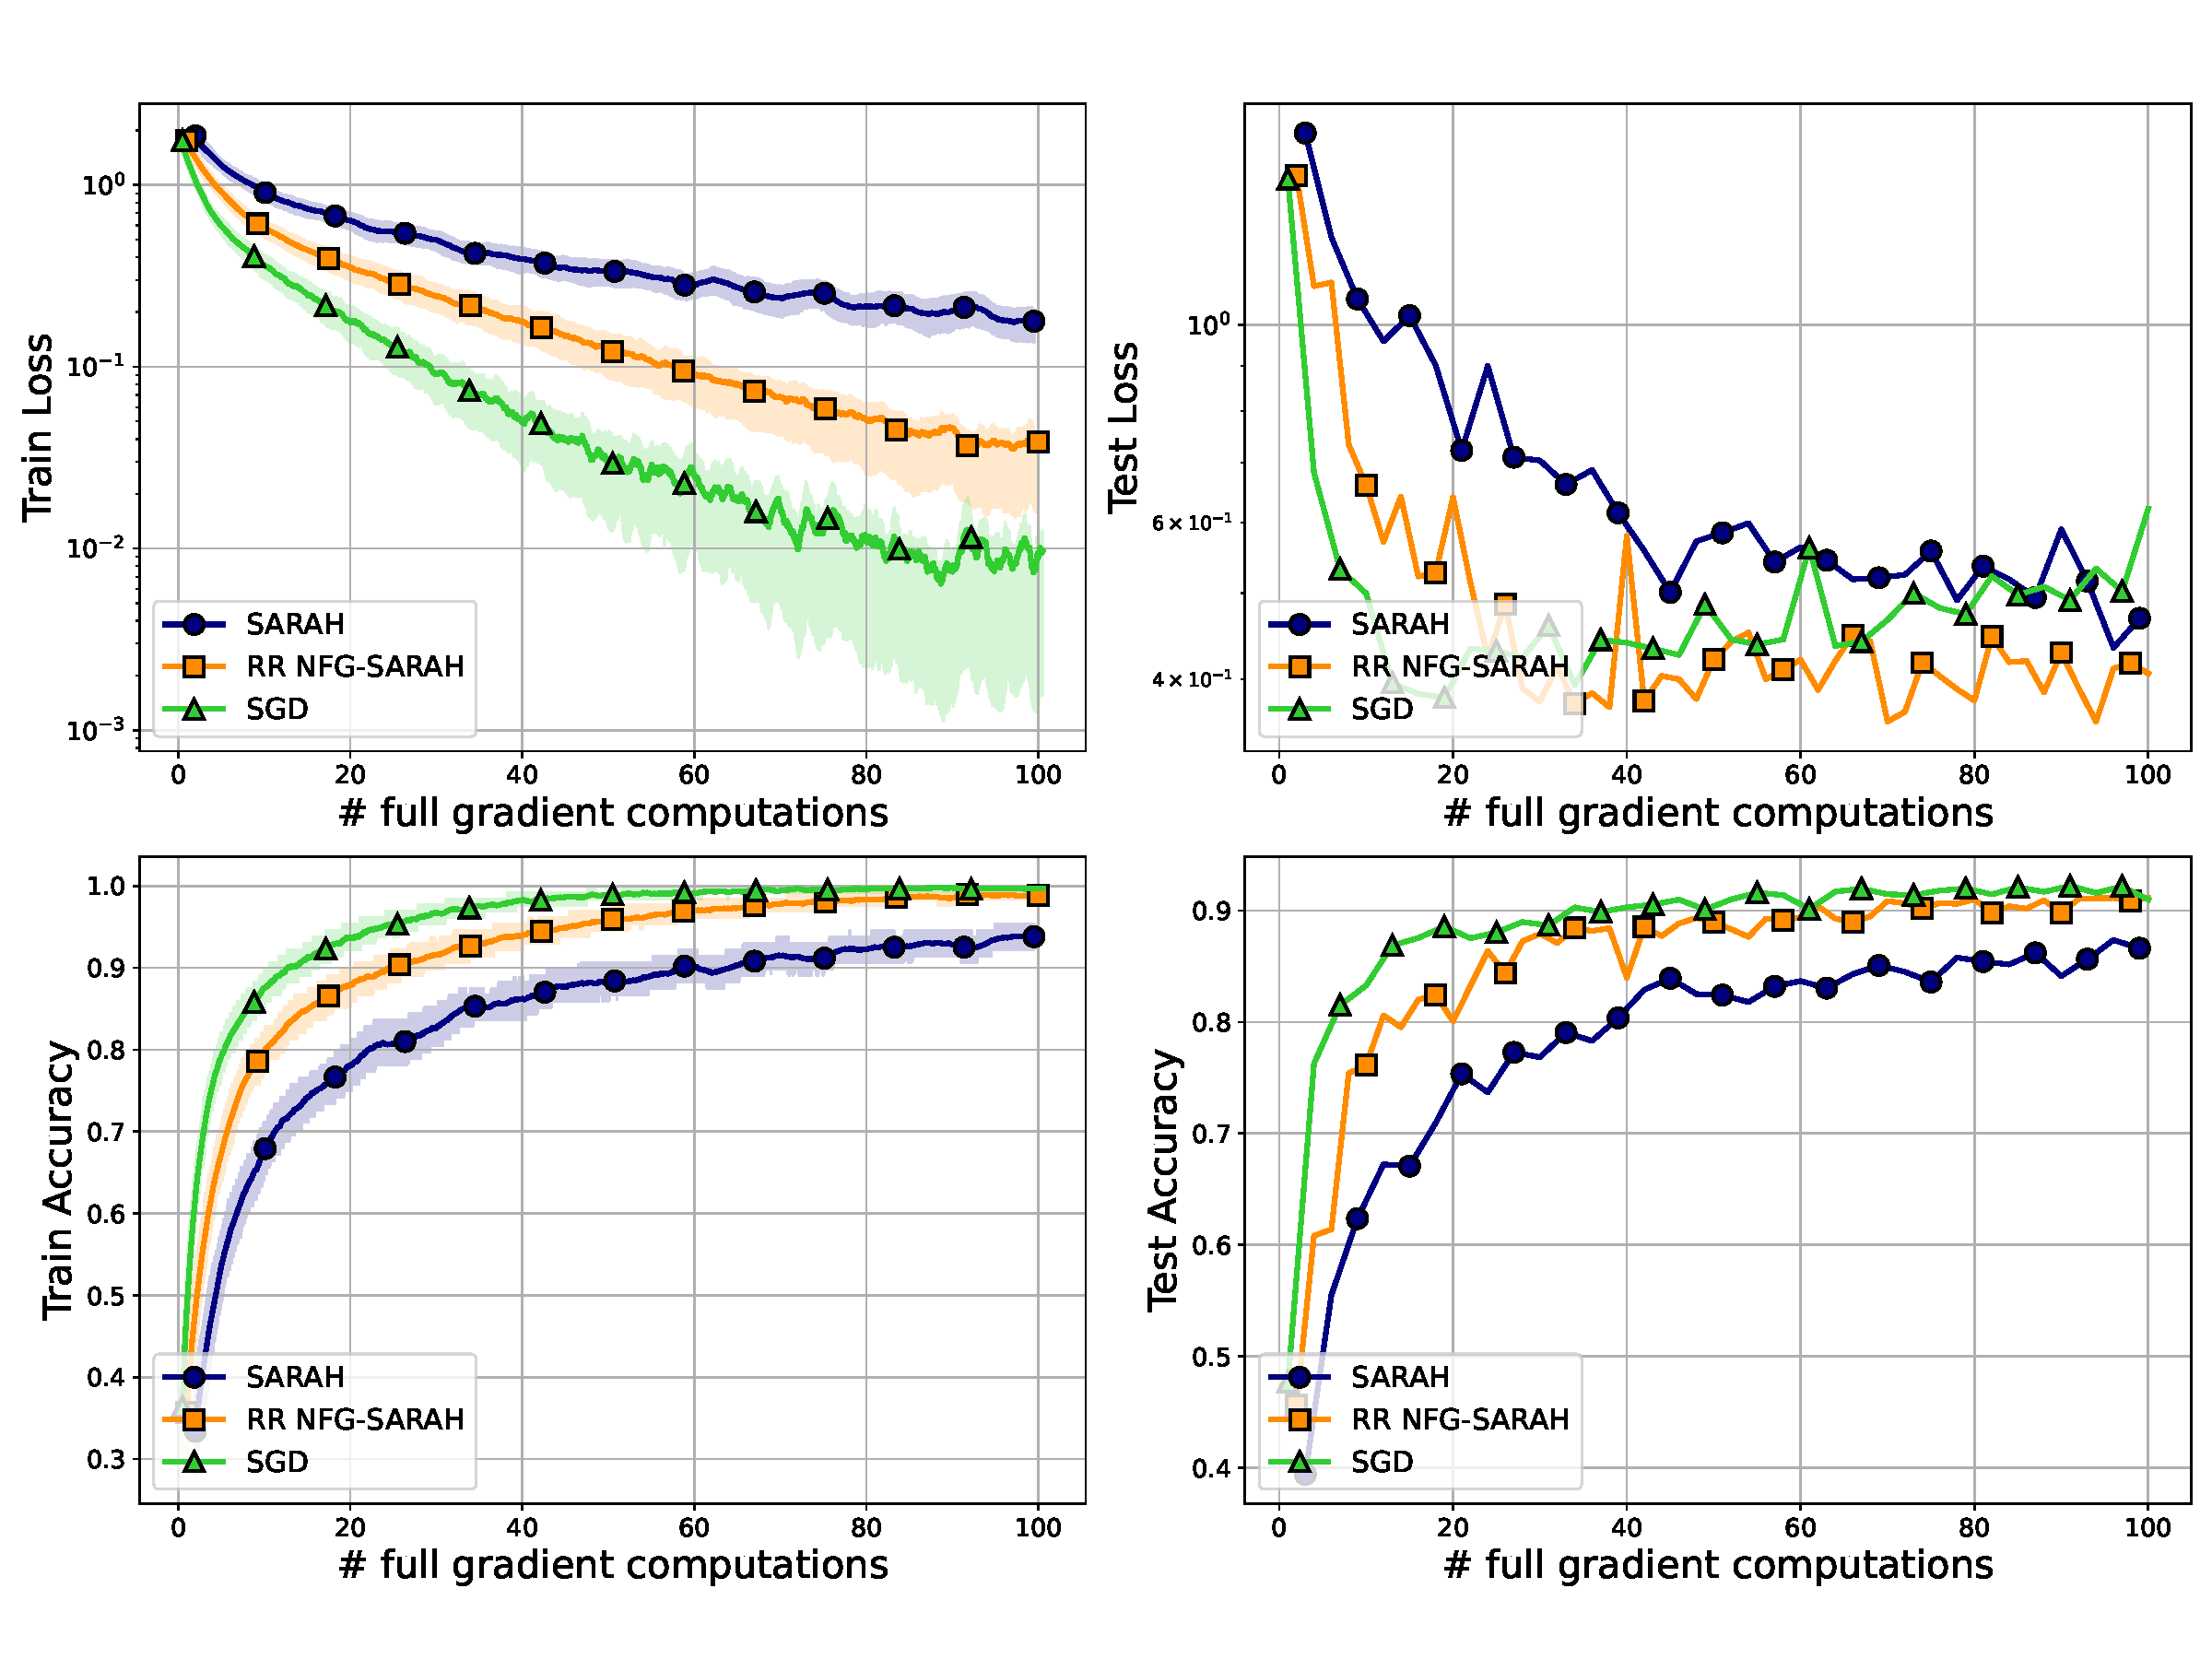
\includegraphics[width=\linewidth]{../figures/sarah_10.pdf}
\end{figure}
\end{frame}

\begin{frame}{Эксперимент: CIFAR-100 + ResNet18}
    Задача многоклассовой классификации на датасете CIFAR-100:
    \begin{itemize}
        \item 60\,000 изображений $32\times32$
        \item 100 классов (по 600 изображений на класс)
    \end{itemize}

    Используется архитектура ResNet-18.

    Функция потерь — кросс-энтропия:
    \[
    \min\limits_{w} \frac{1}{M} \sum_{i=1}^{M} \ell(f_w(x_i), y_i),
    \]
    где $w$ — параметры модели, $f_w(x_i)$ — выход модели, $y_i$ — метка, $\ell$ — кросс-энтропия.

    Метод \textsc{No Full Grad SARAH} сравнивается с классическим \textsc{SARAH}.
\end{frame}

\begin{frame}{Графики: CIFAR-100}
\begin{figure}
\centering
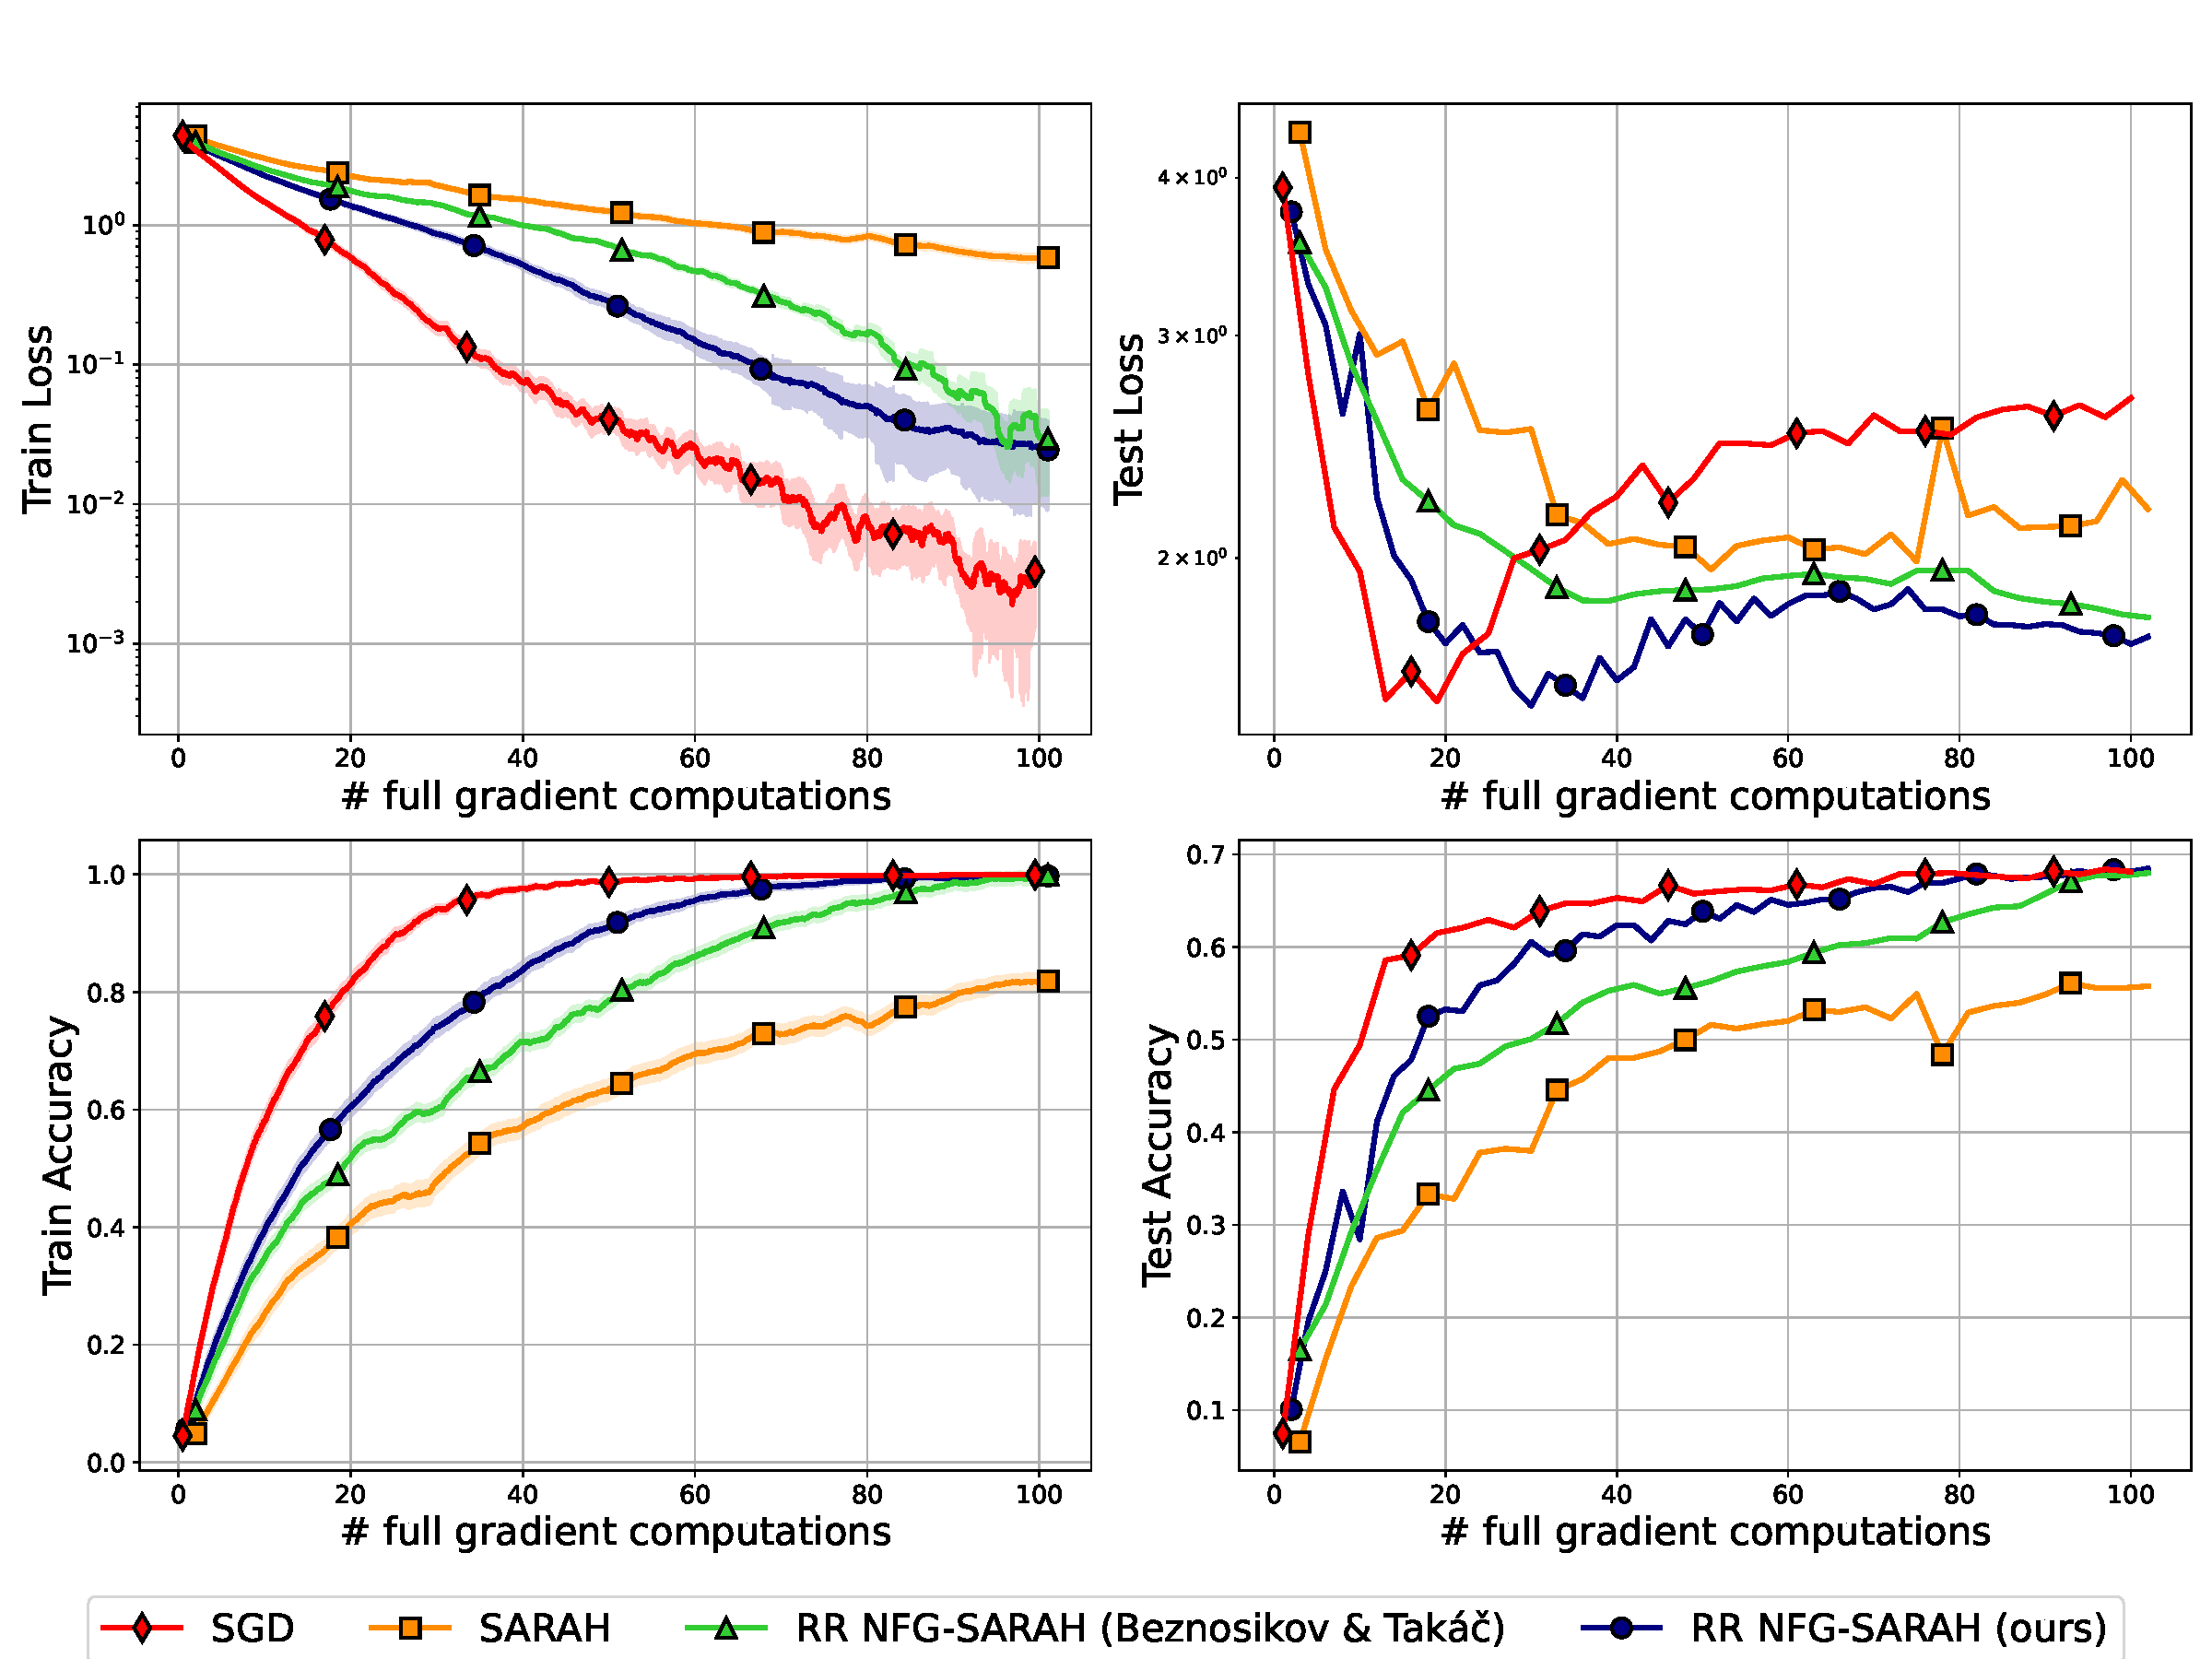
\includegraphics[width=\linewidth]{../figures/CIFAR100_LR=0.7_plots_compressed.pdf}
\end{figure}
\end{frame}

\begin{frame}{Эксперимент: Tiny ImageNet + Swin Transformer}
    Задача классификации изображений на Tiny ImageNet:
    \begin{itemize}
        \item 200 классов, изображения $64\times64$
        \item масштабирование до $224\times224$ для Swin
    \end{itemize}

    Используется модель Tiny Swin Transformer (\texttt{swin\_T\_patch4\_window7\_224}), инициализированная предобученными весами с ImageNet-1K.

    Размер батча: 256, градиентный клиппинг: 1.0. Метрики: точность и кросс-энтропия. Сравниваются методы: \textsc{SGD}, \textsc{SARAH}, RR \textsc{NFG-SARAH}, предложенный \textsc{No Full Grad SARAH}.
\end{frame}

\begin{frame}{Графики: Tiny ImageNet}
\begin{figure}
\centering
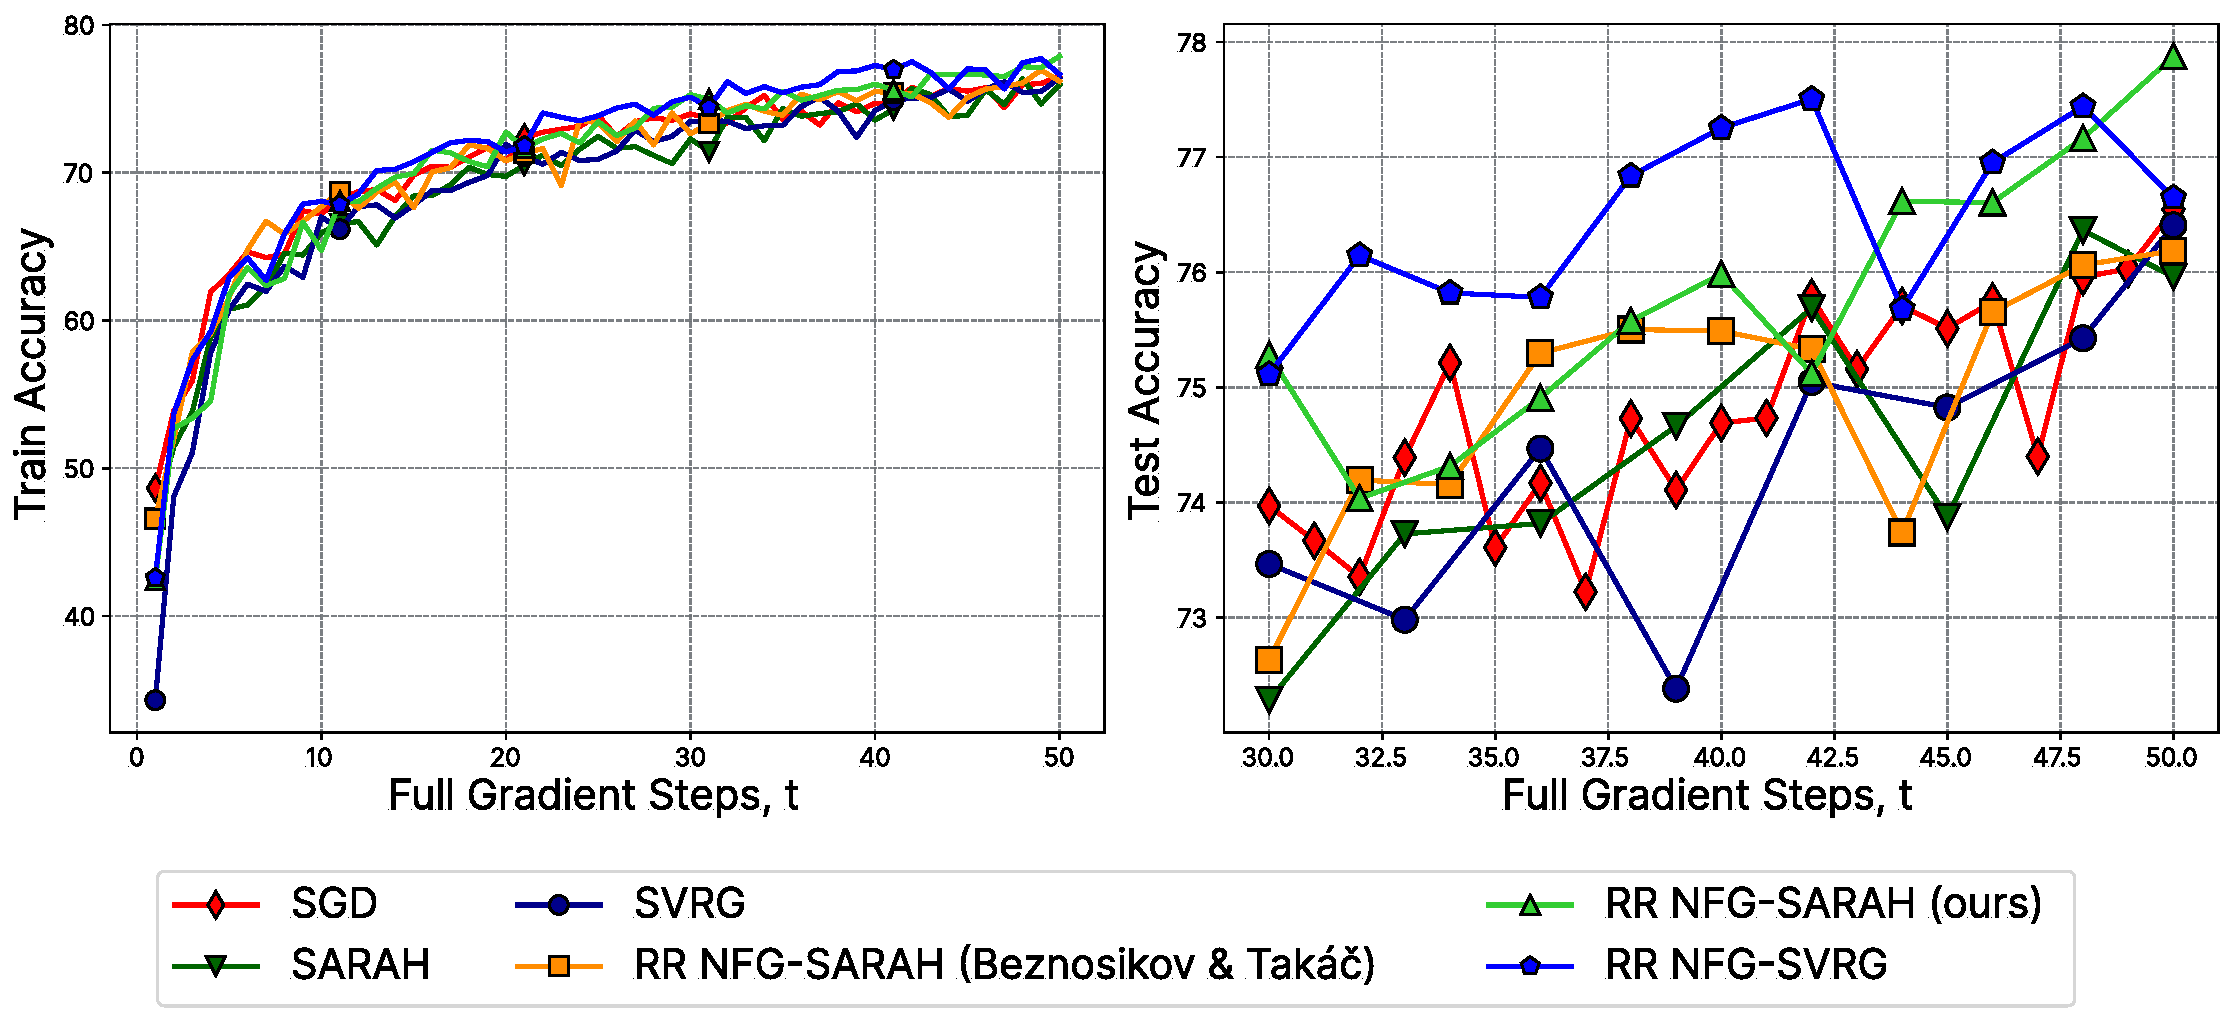
\includegraphics[width=\linewidth]{../figures/vit_results.pdf}
\end{figure}
% \begin{table}
% \centering
% \begin{tabular}{l|c}
% \toprule
% Метод & Точность ($\uparrow$) \\
% \midrule
% \textsc{SGD} & 76.545 \\
% \textsc{SARAH} & 75.961 \\
% RR \textsc{NFG-SARAH} () & 76.186 \\
% RR \textsc{NFG-SARAH} (предложенный) & \textbf{77.875} \\
% \bottomrule
% \end{tabular}
% \end{table}
\end{frame}


% 7. Выводы для защиты
\begin{frame}{Выносится на защиту}
    \begin{itemize}
        \item Предложен новый вариант метода  \textbf{SARAH}, не использующий вычисление полного градиента.
        \item Использование перемешивания и скользящего среднего позволило аппроксимировать полный градиент без дополнительной памяти.
        \item Методы обладают улучшенными 
        \begin{itemize}
            \item \textbf{Затратами памяти:} требуется \(\order{d}\) вместо \(\order{nd}\)
            \item \textbf{Сходимостью:} лучшие оценки по числу итераций
        \end{itemize}
        \item Проведены эксперименты (CIFAR-10/CIFAR-100 + ResNet18 и Tiny ImageNet + Swin Transformer), подтверждающие теоретические преимущества.
    \end{itemize}
    \end{frame}
    

    
\end{document}
